\subsection{Использование грида}
\label{sec:manual:grid_manual}

Компонент грид-разметки представлят собой ни что иное, как место, куда пользователь будет перетягивать компоненты, передвигать, настраивать и т.д. Это главный инструмент данного программного средства, позицинирование элементов на нем осуществляется при помощи смещения относительно начала координат: верхней левой точки грида.

Перемещение элементов зависит от размера сетки: чем мельче сетка, тем меньше шаг, с которым могут быть передвинуты компоненты. Ее размер редактируется при помощи панели инструментов, находяшейся сверху:

\begin{figure}[ht]
  \centering
    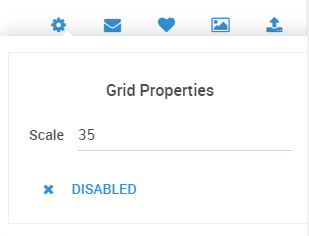
\includegraphics[scale=0.5]{manual_grid_tools.png}
    \caption{Инструмент настройки размеров сетки грида}
    \label{sec:manual:manual_grid_tools}
\end{figure}

Также при помощи кнопки <<DISABLED/ENABLED>> можно выключать/включать отображение сетки.

Сама сетка изначально имеет размер 20 пикселей. Результат изменения размера сетки предсавлен на рисунке~\ref{sec:manual:manual_using_grid_tools}.

\begin{figure}[ht]
  \centering
    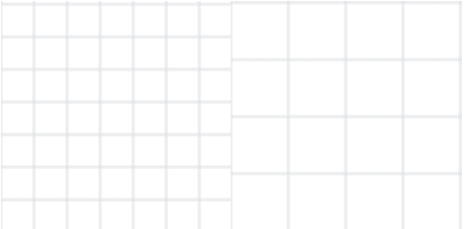
\includegraphics[scale=0.5]{manual_using_grid_tools.png}
    \caption{Результат изменения размеров сетки грида}
    \label{sec:manual:manual_using_grid_tools}
\end{figure}

